\documentclass[12pt]{article}
\usepackage{amsmath}
\usepackage{graphicx}
\usepackage{hyperref}
\usepackage[utf8]{inputenc}
\usepackage{listings, wrapfig}
\usepackage{color, geometry}
\geometry{a4paper, top=3cm, bottom=3cm, left=3.5cm, right=3.5cm}
\title{Report Finale: Track My Pantry}
\author{Marco Benito Tomasone 873909}
\date{04/09/2021}

\definecolor{dkgreen}{rgb}{0,0.6,0}
\definecolor{gray}{rgb}{0.5,0.5,0.5}
\definecolor{mauve}{rgb}{0.58,0,0.82}

\lstset{frame=tb,
  language=Java,
  aboveskip=3mm,
  belowskip=3mm,
  showstringspaces=false,
  columns=fullflexible,
  basicstyle={\small\ttfamily},
  numbers=left,
  numberstyle=\tiny\color{gray},
  keywordstyle=\color{blue},
  commentstyle=\color{dkgreen},
  stringstyle=\color{mauve},
  breaklines=true,
  breakatwhitespace=true,
  tabsize=1
}
\begin{document}
\maketitle
\section{Introduzione}
    Questo documento è parte integrante del progetto finale del corso di Laboratorio di Applicazioni Mobili, dell'Alma Mater Studiorum - 
    Università di Bologna, dell'A.S. 2020/2021. \\
    Il progetto prevedeva la produzione di un'applicazione che permetteva ai suoi utenti di tenere traccia dei prodotti nella propria dispensa 
    e di creare un database collaborativo di barcode di prodotti e delle loro caratteristiche.
    Questo report finale è una rendicontazione del lavoro svolto, una spiegazione delle scelte implementative ed una presentazione delle 
    feature prodotte.
\section{Feature del Progetto}
\subsection{Requisiti Minimi}
    Le feature ufficialmente richieste, e minime, per questo progetto sono principalmente due:
    \begin{itemize}
        \item \textbf{Migliorare il database collaborativo: } tutti gli utenti dell'applicazione devono essere in grado di partecipare alla
        costruzione di un database collaborativo e collettivo, in cui gli utenti possono cercare i loro prodotti inserendo il barcode , inserirne
        di nuovi nel caso non fossero presenti ed esprimere una loro valutazione positiva relativamente ad un prodotto in particolare. Per 
        accedere a questo database gli utenti devono essere in grado di registrarsi e di autenticarsi correttamente al database.
        \item \textbf{Tenere traccia dei prodotti nella dispensa: } tutti i prodotti ottenuti/inseriti dal database collaborativo devono essere correttamente
        inseriti in un database locale che deve permettere agli utenti di tenere traccia dei prodotti in loro possesso ed eliminarli a fine utilizzo.
    \end{itemize}
\subsection{Feature Aggiuntive}
    Particolarmente indicata era la possibilità di inserire delle feature aggiuntive al progetto. Qui di seguito la lista delle feature da me aggiunte:
    \subsubsection{Categorie}
    La prima feature aggiuntiva che ho inserito nel progetto è una divisione dei prodotti per categorie. L'utente può inserire e gestire i
    prodotti in una categoria particolare, es. Carne, Pesce, Lievitati, Dolci, Bevande. Si potrebbe anche pensare ad un utilizzo delle categorie per 
    macronutrienti, quindi carboidrati, grassi e proteine. Le operazioni possibili sulle categorie sono: inserimento, modifica ed eliminazione.
    \subsubsection{Quantità dei prodotti}
    La seconda feature aggiuntiva è stata l'aggiunta della quantità dei prodotti. Al momento dell'inserimento di un nuovo prodotto la quantità
    base è pari ad 1. Successivamente è possibile aumentarne e diminuirne la quantità durante la visualizzazione della propria dispensa.
    Dal momento in cui la quantità di un prodotto scende a 0, il prodotto non viene eliminato dal database ma viene inserito nella Lista Della Spesa.
    \subsubsection{Scansionamento del Barcode}
    Oltre che inserire il barcode manualmente è possibile scansionare il barcode tramite la fotocamera ed attivare il flash durante la scansione
    premendo il tasto Volume Su.
    \subsubsection{Filtrare i prodotti per nome}
    Durante la visualizzazione della lista dei prodotti per categoria è possibile tramite un'apposita barra di ricerca filtrare i prodotti 
    per nome, carattere per carattere durante l'inserimento. 
    \subsubsection{Immagini}
    Per i prodotti nel database collaborativo per i quali è stata inserita un'immagine è possibile visualizzarla in tutte le parti dell'applicazione 
    in cui è prevista la visualizzazione del prodotto (Lista dei prodotti, Lista della spesa, Sezione di ricerca del prodotto). Per i prodotti
    per i quali non è stata opportunamente caricata una foto, verrà visualizzata un'immagine fittizzia.
    \subsubsection{Inserimento di un nuovo prodotto scattando una foto}
    Al momento dell'inserimento di un nuovo prodotto nel database collaborativo è possibile scattare una foto del prodotto ed allegarla ad esso
    durante l'inserimento, in modo tale da visualizzarla per tutti i successivi usi del prodotto stesso. L'app è pensata per essere utilizzata in
    semplicità e principalmente scansionando i codici a barre dei prodotti, quindi avendoli fisicamente durante l'utilizzo. E' difficile pensare
    ad un utilizzo dell'applicazione in cui l'utente inserisce il codice a barre manualmente, questo è il motivo per cui è possibile fare una foto
    del prodotto per allegarla ma non è possibile caricarne una dalla galleria.
    \subsubsection{Lista della Spesa}
    Dal momento in cui un prodotto raggiunge una quantità pari a 0, viene eliminato dalla lista dei prodotti ed inserito nella lista della spesa.
    Questa serve come reminder dei prodotti da acquistare in negozio. Dal momento in cui un prodotto viene nuovamente scannerizzato ed inserito
    nella lista dei prodotti viene automaticamente eliminato dalla lista della spesa.
    \subsubsection{Gestione degli utenti}
    Per accedere all'app ed utilizzare il database collettivo viene richiesto un login. La procedura di login viene sfruttata per separare i prodotti
    nel database locale di utenti diversi. E' possibile quindi utilizzare l'applicazione con due utenti diversi ed i prodotti verranno correttamente 
    separati fra i due.\\ \\
    \section{Aspetti Implementativi}
    In questa sezione spiegherò quelle che sono state le scelte implementative del progetto, allegando degli snippet di codice. Durante 
    la stesura di questo progetto è stato utilizzato il pattern Model View View Model (MVVM), il database locale è stato gestito tramite Room, mentre le 
    chiamate alle API del database collaborativo sono state gestite mendiante Retrofit.
    \subsection{SplashActivity}
    Questa è l'activity di caricamento dell'applicazione. E' un'activity prettamente grafica, durante il suo caricamento sceglie quale è la prossima activity
    da invocare. Se il token di login è ancora valido carica direttamente l'activity con la lista delle categorie, altrimenti viene caricata l'activity di login.
    \begin{lstlisting}
    
        int oneWeekAsSec = 604800;
        SharedPreferences pref = getApplication().getApplicationContext().getSharedPreferences("MY_PREFERENCES", Context.MODE_PRIVATE);
        long currentDate = Calendar.getInstance(Locale.getDefault()).getTimeInMillis() / 1000;
        Long savedAccessTokenData = Long.valueOf(pref.getString("DATA", String.valueOf(-1)));
        Intent intent = null;
        if(savedAccessTokenData != -1) {
            if (currentDate < savedAccessTokenData + oneWeekAsSec)
                intent = new Intent(SplashActivity.this, CategoryListActivity.class);
            else{
                Toast.makeText(SplashActivity.this,"Token Expired! Please Log In", Toast.LENGTH_SHORT).show();
                intent = new Intent(SplashActivity.this, LoginActivity.class);
            }
        }
        else
                intent = new Intent(SplashActivity.this, LoginActivity.class);
}
    \end{lstlisting}
    
    La scelta di usare per i dati della login le SharedPreferences e non magari il database è data dalla volontà di sperimentare più soluzioni possibili
    per apprendere il più possibile. Può succedere infatti che delle scelte implementative per questo progetto non siano le migliori e che avrei potuto fare
    scelte diverse, la ragione è proprio quella di sperimentare il più possibile con il codice.\\
    \subsection{Login \& registrazione }
    \begin{wrapfigure}{l}{4cm}
        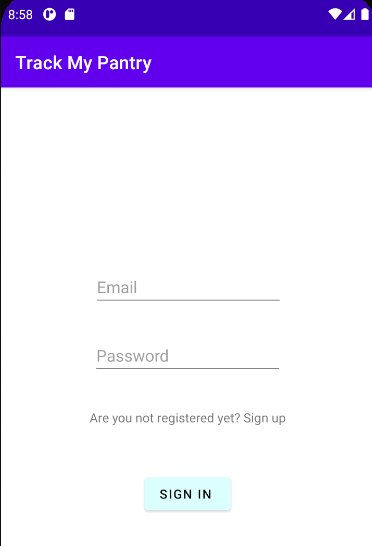
\includegraphics[width=3.5cm]{img/Login.PNG}
    \end{wrapfigure}
    L'activity di Login e Registrazione contiene un campo nascosto il campo name, che viene visualizzato o meno nel momento in cui si preme il testo per 
    passare tra una vista e l'altra. Questa activity ha un view Model che si occupa di gestire le richieste. Il view model è composto da solo due chiamate
    la login e la register ed esso sono associati delle classi opportunamente create per la gestione dei dati richiesti, come la LoginData e la RegisterData.\\
    \subsection{Database \& chiamate http}
    In entrambe le classi per la gestione del database con Room e per la gestione delle chiamate Http con Retrofit è stato utilizzato il design pattern creazionale 
    Singleton. 
    \begin{lstlisting}
        @Database(entities = {Category.class, Product.class}, version = 10)
public abstract class AppDataBase extends RoomDatabase {
    public abstract PantryDao pantryDao();

    public static AppDataBase INSTANCE;

    public static AppDataBase getDataBaseInstance(Context context){
        if(INSTANCE == null){
            //create the database
            INSTANCE = Room.databaseBuilder(context.getApplicationContext(), AppDataBase.class, "ProductDatabase")
                    .fallbackToDestructiveMigration()
                    .build();
        }
        return INSTANCE;

    }
}
    \end{lstlisting}
    Allego solo il codice della classe AppDataBase dal momento in cui la classe RetroIstance è simile. Per il DB è stata creata poi una interfaccia DAO, mentre 
    per Retrofit è stata creata un'interfaccia per i Service HTTP. Allego in questo caso la seconda.
    \begin{lstlisting}
        public interface APIService {
    @Headers("Content-Type: application/json")
    @POST("users")
    Call<Authentication> registrationMethod(@Body RegisterData registerData);

    @Headers("Content-Type: application/json")
    @GET("users/me")
    Call<Authentication> getUserData(@Header("Authorization") String accessToken);

    @Headers("Content-Type: application/json")
    @POST("auth/login")
    Call<AccessToken> loginMethod(@Body LoginData loginData);

    @Headers("Content-Type: application/json")
    @POST("products")
    Call<Product> insertNewProduct(@Body CreateProductSchema product, @Header("Authorization") String accessToken);

    @Headers("Content-Type: application/json")
    @GET("products")
    Call<GetProductSchema> getProductByBarcode(@Query("barcode") String Barcode, @Header("Authorization") String accessToken);

    @Headers("Content-Type: application/json")
    @POST("votes")
    Call<Void> insertVote(@Body CreateVoteSchema voteSchema, @Header("Authorization") String accessToken);
}
    \end{lstlisting}
    \subsection{Activity Categorie}
    Per la gestione delle categorie è stata creata una tabella apposita all'interno del database. La gestione grafica delle 
    categorie è affidata ad una Recycler View. Utilizzando il pattern MVVM, a questa classe sono collegati un ViewModel ed un 
    Adapter che servono per la gestione delle categorie.
    Il view model è così fatto:
    \begin{lstlisting}
        public class CategoryListViewModel extends AndroidViewModel {

    private MutableLiveData<List<Category>> listOfCategories;
    private AppDataBase appDataBase;
    private SharedPreferences pref;

    public CategoryListViewModel(Application application){
        super(application);
        listOfCategories = new MutableLiveData<>();
        appDataBase = AppDataBase.getDataBaseInstance(getApplication().getApplicationContext());
        pref = getApplication().getApplicationContext().getSharedPreferences("MY_PREFERENCES", Context.MODE_PRIVATE);
        getAllCategories();
    }
    //Observer for the liveData, so for the categories you have
    public MutableLiveData<List<Category>> getListOfCategoriesObserver(){
        return listOfCategories;
    }

    //Function to get all the categories in the DataBase and post them into the liveData
    public void getAllCategories(){
        List<Category> categoriesList = appDataBase.pantryDao().getAllCategories(pref.getString("EMAIL", null));
        if(categoriesList.size() > 0)
            listOfCategories.postValue(categoriesList);
        else
        listOfCategories.postValue(null);
        }
        public void insertCategory(String categoryName){    
            }
    public void updateCategory(Category category){    
        }
        public void deleteCategory(Category category){  
            }
}
\end{lstlisting}
Il codice delle funzioni non è stato inserito per semplicità dal momento in cui verrà allegato a questo report.
La particolarità principale è il MutableLiveData che permette di essere aggiornato tramite quell'Observer
ed essere osservato dall'Adapter che permette un aggiornamento automatico all'applicazione delle operazioni
come inserimento, modifica ed eliminazione di una categoria. Dal momento in cui si decide di eliminare una categoria
    dal proprio database verranno anche contestualmente eliminati tutti i prodotti in essa contenuti. La modifica permette,
    invece, di cambiare il nome della categoria. Il campo email che viene passato alla funzione getAllCategories() serve
    per ottenere solo i prodotti di un determinato utente, stessa cosa verrà fatta per i prodotti. 
    Per semplicità dell'Adapter verranno riportate solo tre parti di codice: 
    \begin{lstlisting}
        public void setCategoryList(List<Category> categoryList){
            this.categoryList = categoryList;
            notifyDataSetChanged();
            }
    \end{lstlisting}
    La prima è questa funzione che serve per notificare alla View che i dati sono cambiati e di conseguenza riaggiornare la view.
    \begin{lstlisting}
        
        @Override //Set data to our TextView
        public void onBindViewHolder(@NonNull CategoryListAdapter.MyViewHolder holder, int position) {
            holder.tvCategoryName.setText(this.categoryList.get(position).categoryName);
            
            holder.itemView.setOnClickListener(new View.OnClickListener() {
                @Override
                public void onClick(View v) {
                    clickListener.itemClick(categoryList.get(position));
                }
                });
                
                holder.editCategory.setOnClickListener(new View.OnClickListener() {
                @Override
                public void onClick(View v) {
                    clickListener.editClick(categoryList.get(position));
                }
                });
                
                holder.deleteCategory.setOnClickListener(new View.OnClickListener() {
                    @Override
                    public void onClick(View v) {
                        clickListener.deleteClick(categoryList.get(position));}});}
    \end{lstlisting}    
    Questa funzone serve invece per fare binding tra i dati e le parti della View. Come è possibile vedere
    implementano delle funzioni di un clickListener, questo è proprio il dataType sottostante, il ViewHolder. 
    Ce ne saranno di simili per la lista della spesa e per la lista dei prodotti.
    \begin{lstlisting}
        
        public class MyViewHolder extends RecyclerView.ViewHolder{
            TextView tvCategoryName;
            ImageView deleteCategory;
            ImageView editCategory;
                            
            public MyViewHolder(View view){
                super(view);
                tvCategoryName = view.findViewById(R.id.textViewCategoryName);
                deleteCategory = view.findViewById(R.id.image_delete_category);
                editCategory = view.findViewById(R.id.image_edit_category);
                }
                }
                
                public interface HandleCategoryClick {
                    void itemClick(Category category);
            void deleteClick(Category category);
            void editClick(Category category);}}
        \end{lstlisting}
        \begin{wrapfigure}{l}{3.5cm}
            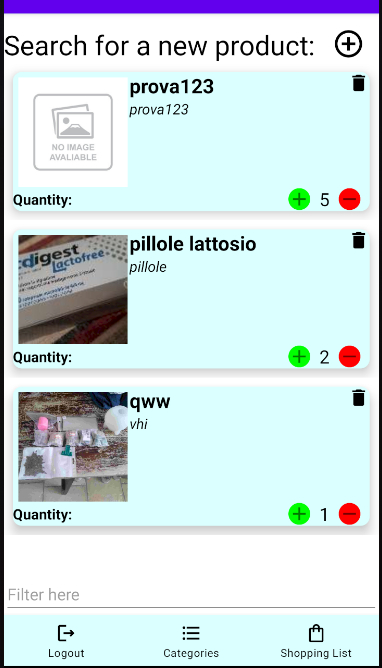
\includegraphics[width=3.5cm]{img/productlist.PNG}
        \end{wrapfigure}
    \subsection{Activity Lista di Prodotti}
    Per la lista dei prodotti l'architettura è simile che per la gestione delle categorie, c'è quindi il ViewModel,
    l'Adapter, ma, in aggiunta è stato utilizzato il pattern Repository per implementare la SingleSource of Truth.
    In questo caso quindi il View Model si occupa di collegare le chiamate della view al Repository che al contrario    
    si occupa delle chiamate e della consistenza dei dati nel db interno. Il Repository è unico per tutti i prodotti, sia 
    quelli nella lista della spesa che per quelli nella lista dei prodotti. Si allega ad esempio la funzione per la creazione di
    un nuovo prodotto. A seguito di una chiamata http con successo il prodotto oltre ad essere inserito nel db collaborativo
    viene anche automaticamente inserito nel database locale dell'utente.
    \\\\
    \begin{lstlisting}
        public void createNewProduct(CreateProductSchema productSchema, int categoryId, SearchProductsActivity searchProductsActivity) {
        APIService apiService = RetroInstance.getRetroClient().create(APIService.class);
        Call<Product> call = apiService.insertNewProduct(productSchema, "Bearer " + pref.getString("ACCESS_TOKEN",""));
        call.enqueue(new Callback<Product>() {
            @Override
            public void onResponse(Call<Product> call, Response<Product> response) {
                if (response.isSuccessful()) {
                    Product product = (Product) response.body();
                    product.setCategoryId(categoryId);
                    product.setUserEmail(pref.getString("EMAIL", null));
                    insertProduct(product);
                } else{
                    Toast.makeText(searchProductsActivity.getApplicationContext(),"Error creating Product!", Toast.LENGTH_SHORT).show();
                }
            }
            @Override
            public void onFailure(Call<Product> call, Throwable t) {
                Log.e("ERROR", t.getMessage());
            }
        });
    }
    \end{lstlisting}
    \subsection{Filtrare i prodotti}
    Il filtro dei prodotti per nome è stato semplicemente implementato mediante una TextView e ad ogni carattere inserito
    tramite un textwatcher viene chiamata una funzione dell'adapter per cercare e mostrare i prodotti contenenti quella sottostringa
    tra tutti i prodotti posseduti in quella categoria.
    \begin{lstlisting}
        public void afterTextChanged(Editable s) {
            filterList(s.toString());}
    \end{lstlisting}
    \subsection{Ricerca di un prodotto}
    \begin{wrapfigure}{l}{3.5cm}
        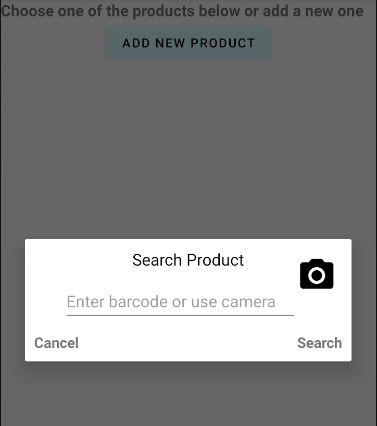
\includegraphics[height=3.5cm]{img/search.PNG}
    \end{wrapfigure}
    La ricerca di un prodotto viene fatta tramite le chiamate, al ritorno da una ricerca si ottiene la lista di tutti i prodotti con 
    quel barcode. Se si clicca su un prodotto questo viene aggiunto alla lista dei prodotti nel database locale, ma prima viene chiesto di 
    darne una valutazione da 1 a 5 stelle, tramite una rating bar.
    \\\\\\
    \subsection{Inserimento di un nuovo prodotto}
    Se non si è trovato prodotti che rispecchiano i parametri di ricerca è possibile inserirne di nuovi, l'inserimento di un nuovo prodotto
    tramite l'apposito button richiederà il nome, la descrizione di un prodotto ed eventualmente è possibile scattare una foto al prodotto tramite 
    la fotocamera. Se si tenta di inserire un prodotto che è già inserito il prodotto vedrà aumentare la sua quantità di 1. Se si tenta di inserire un
    prodotto che già è presente in un altra categoria il prodotto verrà spostato nella nuova catogoria. Se si inserisce un prodotto che era nella 
    shoppinglist verrà rimosso da quest'ultima. Questo meccanismo è stato implementato tramite una piccola query al database che verifica se un prodotto 
    è già al suo interno o meno.
    \begin{lstlisting}
        camera.setOnClickListener(new View.OnClickListener() {
            @Override
            public void onClick(View v) {
                if (ContextCompat.checkSelfPermission(SearchProductsActivity.this, Manifest.permission.CAMERA) != PackageManager.PERMISSION_GRANTED) {
                    ActivityCompat.requestPermissions(SearchProductsActivity.this, new String[]{
                            Manifest.permission.CAMERA}, 100);
                    };
                Intent intent = new Intent(MediaStore.ACTION_IMAGE_CAPTURE);
                startActivityForResult(intent, 100);

            }
        });

        protected void onActivityResult(int requestCode, int resultCode, Intent data) {
            super.onActivityResult(requestCode, resultCode, data);
            if(requestCode == 100){
                Bitmap bitmap = (Bitmap) data.getExtras().get("data");
                imageView.setImageBitmap(bitmap);
                String base64conversion = encodeImage(bitmap);
                base64 = "data:image/jpeg;base64," + base64conversion; }
    \end{lstlisting}
    \subsection{Scanning Barcode Fotocamera}
    E' possibile scannerizzare il barcode dei prodotti con la fotocamera cliccando su un'icona nel dialog di ricerca.
    Il codice per renderlo possibile:
    \begin{lstlisting}
        camera.setOnClickListener(new View.OnClickListener() {
            @Override
            public void onClick(View v) {
                dialogBuilder.dismiss();
                IntentIntegrator intentIntegrator = new IntentIntegrator(SearchProductsActivity.this);
                intentIntegrator.setCaptureActivity(ScanActivity.class);
                intentIntegrator.setDesiredBarcodeFormats(intentIntegrator.ALL_CODE_TYPES);
                intentIntegrator.setBeepEnabled(true);
                intentIntegrator.setOrientationLocked(true);
                intentIntegrator.setPrompt("For Flash use volume up Key");
                intentIntegrator.initiateScan();
            }
        });
    \end{lstlisting}
    \subsection{Immagini dei prodotti}
    Le immagini dei prodotti sono state caricate mediante la libreria Glide. Se l'immagine c'è viene correttamente visualizzata
    altrimenti viene visualizzata un'immagine con il testo "No image avaible". Questa scelta si pone in essere dal momento in cui
    in un utilizzo meno accademico e più reale dell'applicazione, pochi saranno i prodotti non accompagnati da un'immagine.
    \begin{lstlisting}
    if (this.productList.get(position).getImg() != null) {
        if (!this.productList.get(position).getImg().startsWith("data:image/jpeg;base64,"))
            this.productList.get(position).setImg("data:image/jpeg;base64," + this.productList.get(position).getImg());
        Glide.with(context).load(this.productList.get(position).getImg())
        .apply(RequestOptions.centerCropTransform()).into(holder.productImage);
        } else
        Glide.with(context).load(R.drawable.no_image_avaible).into(holder.productImage);
    \end{lstlisting}
    \begin{wrapfigure}{r}{3.5cm}
        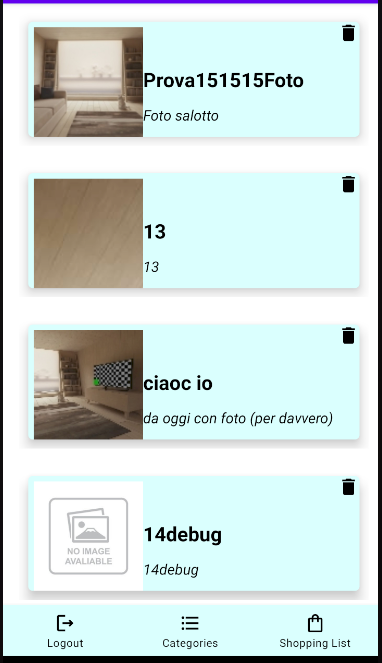
\includegraphics[width=3.5cm]{img/shoppinglist.PNG}
    \end{wrapfigure}
    \subsection{Lista della spesa}
    La lista della spesa è implementata sempre tramite una RecyclerView che visualizzerà tutti i prodotti con quantità
    pari a 0. Anch'essa un Adapter  e si appoggia al ViewModel dei prodotti che ritorna un observer per i soli prodotti che hanno un quantità 
    pari a 0. Il tasto delete nella lista della spesa elimina un prodotto nel database locale, mentre se si riacquista un prodotto
    che è nella lista della spesa viene tolto da quest'ultima e inserito nella categoria di appartenenza.
    \\\\\\\\\\\\\\

    \section{Conclusioni}
    Il progetto è stato molto utile per affacciarmi e imparare delle nuove tecnologie che non avevo mai sperimentato prima.
    Probabilemte non tutte le scelte sono state corrette a livello tecnico ma molte sono state prese per diversificare e sperimentare
    con una nuova tecnologia e cercare di apprendere il più possibile. 
    \end{document}